\documentclass[11pt]{beamer}
\usepackage[utf8]{inputenc}
\usepackage[T1]{fontenc}
\usepackage{amsmath}
\usepackage{amsfonts}
\usepackage{amssymb}
\usepackage{graphicx}
\graphicspath{{Images/}}
\usetheme{default}
\begin{document}
	\author{Cibin Joseph}
	\title{Wake Modelling\\ using the Prescribed Wake Method}
	%\date{}
	%\setbeamertemplate{navigation symbols}{}
	\begin{frame}[plain]
	\maketitle
\end{frame}

\begin{frame}[t]
\frametitle{Wake/Fluid Modelling}
\begin{columns}[t]
	\begin{column}{0.5\textwidth}
		\textbf{Eulerian-based}
		\begin{itemize}
			\item Conventional CFD
			\vspace{2.2cm}
			\begin{figure}
				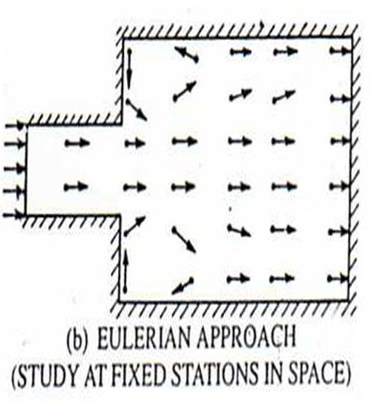
\includegraphics[scale=0.4]{Euler.jpg}
			\end{figure}
		\end{itemize}
	\end{column}
	\begin{column}{0.5\textwidth}
		\textbf{Lagrangian-based}
		\begin{itemize}
			\item Vortex filament method
			\begin{itemize}
			\item \alert{Prescribed wake}
			\item Free wake
			\end{itemize}
			\item Vortex particle method
			\item Lattice-Boltzmann CFD
			\begin{figure}
				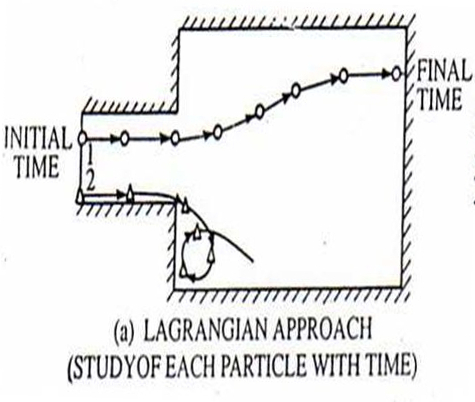
\includegraphics[scale=0.38]{Lagrange.jpg}
			\end{figure}
		\end{itemize}
	\end{column}
\end{columns}
\end{frame}

\begin{frame}[t]
\frametitle{Observations}
\framesubtitle{Wake In Hover}
	\begin{figure}
		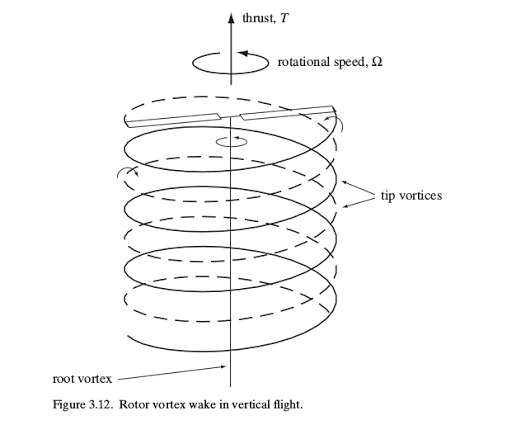
\includegraphics[scale=0.4]{helical_vortex.png}
	\end{figure}
{\tiny Source: W. Johnson, Rotorcraft Aeromechanics}
\end{frame}

\begin{frame}[t]
\frametitle{Landgrebe wake model for Hover}
\begin{align}
	\bar{r}_{tip} &=\alert{A}+(1-\alert{A})exp(-\alert{\Lambda} \psi_w)\\
	\bar{z}_{tip} &=\alert{k_1}\psi_w \hspace{4.5cm} 0\le\psi_w\le 2\pi/N_b\\
	       &=\alert{k_1}\frac{2\pi}{N_b}+\alert{k_2}(\psi_w-\frac{2\pi}{N_b}) \hspace{1.8cm} \psi_w\ge 2\pi/N_b
\end{align}

\vspace{0.5cm}
Parameters:\\
A=0.78, $\Lambda=0.145+27C_T$
\begin{align*}
	k1 &= -0.25(C_T+0.001\theta_{tw}^o)\\
    k2 &= -(1.41+0.001\theta_{tw}^o)\sqrt{C_T/2}
\end{align*}
\end{frame}

\begin{frame}[t]
\frametitle{Beddoes generalised wake model}
	\begin{equation}
		\lambda_i=\lambda_o(1+E\bar{x}-E|\bar{y}^3|)
	\end{equation}
	\begin{align}
		\bar{x}_{tip}&=r_v\cos\psi_v+\mu\psi_w\\
		\bar{y}_{tip}&=r_v\sin\psi_v\\
		\bar{z}_{tip}&=-\mu\tan\alpha\psi_w+\int_{0}^{\psi_w}\lambda_id\psi
	\end{align}
	{\small Note that, $\psi_v=\psi_b-\psi_w$}\\
	3 cases when evaluating integral term:\\
	\vspace{-0.5cm}
\begin{align*}
if \quad \bar{x}_{tip}<-r_v\cos\psi_v&\alert{\Rightarrow}-2\lambda_o(1+E\cos\psi_v+0.5\mu-E|\bar{y}_{tip}^3|)\psi_w\\
if \quad \cos\psi_v>0&\alert{\Rightarrow}-2\lambda_o(1-E|\bar{y}_{tip}^3|)\psi_w\\
else &\alert{\Rightarrow}-2\lambda_o\bar{x}_{tip}\frac{1-E|\bar{y}_{tip}^3|}{\mu}
\end{align*}
\end{frame}

\begin{frame}
\frametitle{Murakami's correction}
	\begin{figure}
	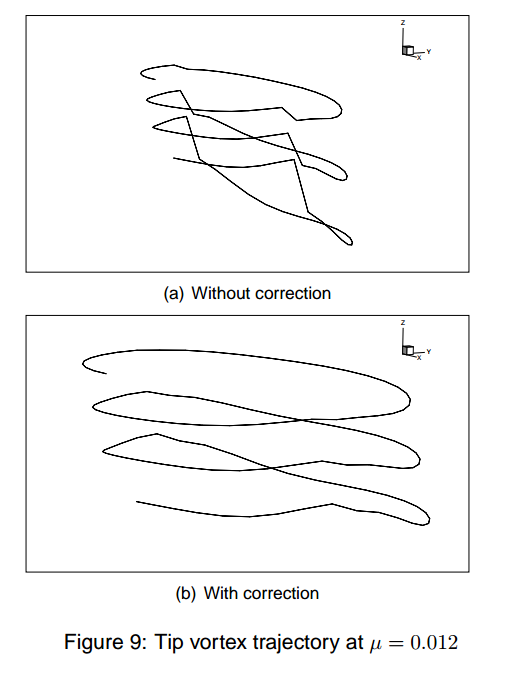
\includegraphics[scale=0.25]{Murakami_correction.png}
\end{figure}
{\tiny Source: G. Reboul. A parametrized BVI noise prediction code. Greener Aviation 2014, Belgium}
\end{frame}
\end{document}